
\documentclass{standalone}
\usepackage[svgnames]{xcolor}
\usepackage{pgfplots}
\pgfplotsset{compat=newest}
\usepackage[sfdefault]{FiraSans}
\usepackage{FiraMono}
\renewcommand*\familydefault{\sfdefault}
\begin{document}
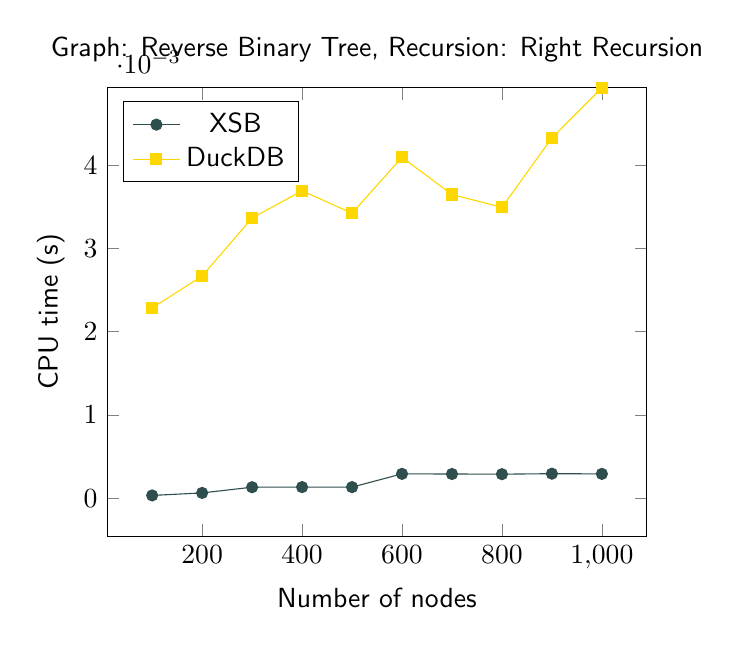
\begin{tikzpicture}
    \begin{axis}[
        title={Graph: Reverse Binary Tree, Recursion: Right Recursion},
        xlabel={Number of nodes},
        ylabel={CPU time (s)},
        legend pos={north west},
        ymax=0.004931799999999986
    ]
    \addplot+[DarkSlateGray, mark options={color=DarkSlateGray}] coordinates {(100,3.2599999999999986e-05) (200,6.280000000000004e-05) (300,0.00013140000000000019) (400,0.00013280000000000003) (500,0.0001323999999999996) (600,0.000292) (700,0.00029019999999999957) (800,0.0002882000000000006) (900,0.0002940000000000002) (1000,0.0002916000000000006)};
\addlegendentry{XSB}
\addplot+[Gold, mark options={color=Gold}] coordinates {(100,0.0022862000000000047) (200,0.0026702) (300,0.0033671999999999925) (400,0.0036937999999999914) (500,0.0034256000000000286) (600,0.0040973999999999846) (700,0.0036495999999999864) (800,0.0034957999999999934) (900,0.0043306000000000065) (1000,0.004931799999999986)};
\addlegendentry{DuckDB}

    \end{axis}
\end{tikzpicture}
\end{document}
